% Compile with:
% latexmk -pdf -pvc -interaction=nonstopmode
%\documentclass[aspectratio=169,10pt,draft]{beamer}
\documentclass[aspectratio=169,10pt]{beamer}
\usetheme{UniBern}
\title{Adaptation Mechanisms Of Zebrafish Respiratory Organ To Endurance Training}
\author{David Haberthür \and
	Dea Aaldijk \and
	Matthias Messerli \and
	Fluri A.\ M.\ Wieland \and
	Oleksiy Khoma \and
	Helena Röss \and
	Ruslan Hlushchuk}
\institute{Institute of Anatomy\\University of Bern\\Switzerland}
\date{June 5, 2019 | \href{https://www.bruker.com/events/micro-ct-users-meeting.html}{Bruker micro-CT Users Meeting 2019}}

%\includeonlyframes{current}
%then....
%\begin{frame}[label=current]
%\end{frame}

\usepackage[english]{babel}
\usepackage{microtype}
\usepackage[backend=biber,
	style=numeric,
	url=false,
	isbn=true,
	maxbibnames=1,
	sorting=none,
	backref=true]{biblatex}
	\addbibresource{../../Documents/library.bib}
\usepackage{graphicx}
\usepackage{tikz}
\usepackage[detect-all=true, range-phrase=--, range-units=single, binary-units=true]{siunitx}
\usepackage[absolute,overlay]{textpos} %for the \source{} command
\usepackage{gitinfo2}
\usepackage[version=4]{mhchem}
\usepackage{xspace}
\usepackage{ccicons}
\usepackage{multimedia}

% Some often used abbreviations
\newcommand{\imsize}{\linewidth} % set global image width
\newcommand{\everyframe}{1} % use only every nth frame for the movies
\newlength\imagewidth % needed for scalebars
\newlength\imagescale % needed for scalebars
\newcommand{\uct}{\si{\micro}CT\xspace} % make our life easier

% Easily fill a frame with the whole image.
% Based on http://tex.stackexchange.com/a/334758/828,
\newcommand{\fullframeimage}[1]{%
	\begin{tikzpicture}[remember picture,overlay]%
		\node[xshift=0,yshift=0] at (current page.center){%
			\includegraphics[width=\paperwidth]{#1}};%		
	\end{tikzpicture}%
}

% Acknowledge images just below them
% Based on https://tex.stackexchange.com/a/206925/828
%\newcommand{\source}[2]{\par\hfill\tiny \href{http://#1}{#1} #2}
% Based on https://tex.stackexchange.com/a/282637
\newcommand{\source}[2]{%
	\raisebox{-1ex}{\makebox[0pt][r]{\tiny \href{http://#1}{#1} #2}}
}

%\raisebox{1pt}{\makebox[0pt][r]{\footnotesize some other text}}


% Define us our custom footer
\defbeamertemplate{footline}{unibe}{%
	\hspace*{0.6cm}%
	v. \href{https://github.com/habi/20190605_BrukerUserMeeting/commit/\gitHash}{\gitAbbrevHash}%
	\hspace*{\fill}%
	\insertframenumber\,/\,\inserttotalframenumber%
	\hspace*{1.2cm}%
	\vskip2pt%
}
\setbeamertemplate{footline}[unibe]

% Format bibliography for beamer
% http://tex.stackexchange.com/a/10686/828
\renewbibmacro{in:}{}
% http://tex.stackexchange.com/a/13076/828
\AtEveryBibitem{%
	\clearfield{journaltitle}
	\clearfield{pages}
	\clearfield{volume}
	\clearfield{number}
	\clearfield{editors}
	\clearlist{editors}
	\clearname{editors}
	\clearfield{issn}
	%\clearfield{year}
	%\clearfield{day}
	%\clearfield{month}
	%\clearfield{endday}
	%\clearfield{endmonth}
}


\begin{document}
% We want no footline on the title page, http://tex.stackexchange.com/a/18829/828 helps
{%
	\setbeamertemplate{footline}{}%
	\begin{frame}%
		\maketitle
	\end{frame}%
}

%\begin{frame}
%	\frametitle{Contents}
%	\tableofcontents
%\end{frame}

\begin{frame}
	\frametitle{Hello!}
	\begin{itemize}
		\item<1-> University of Bern, Switzerland
		\item<1-> Institute of Anatomy
		\item<1-> Group for topographic and clinical Anatomy
		\item<1-> \uct-Team: Ruslan Hlushchuk, David Haberthür, Oleksiy-Zakhar Khoma, Fluri Wieland, Carlos Correa Shokiche
		\item<1-> Biomedical research
		\begin{itemize}
			\item microangioCT~\cite{Hlushchuk2018}: Tumor vasculature, angiogenesis in the heart, musculature
			\item Cancer research: Melanoma
			\item Lung imaging: Tumor detection and classification
			\item Physiology: Zebrafish musculature and gills
		\end{itemize}
		\item<1-> SkyScan 1172 \& 1272 \visible<2->{\& 2214}
	\end{itemize}
\end{frame}

\begin{frame}
	\frametitle{Why?}
	\begin{itemize}
		\item Adaptation of respiratory organ to endurance training
		\item Study \ce{O2} metabolism
	\end{itemize}
\end{frame}

\begin{frame}
	\frametitle{Oxygen pathway}
	\begin{columns}
		\begin{column}{0.618\linewidth}
			\begin{itemize}
				\item<1-> Insects: Spiracles \& Trachea
				\item<2-> Bony fishes: Gills
				\item<3-> Mammals: Lungs
			\end{itemize}
		\end{column}
		\begin{column}{0.382\linewidth}
			\only<1>{%
				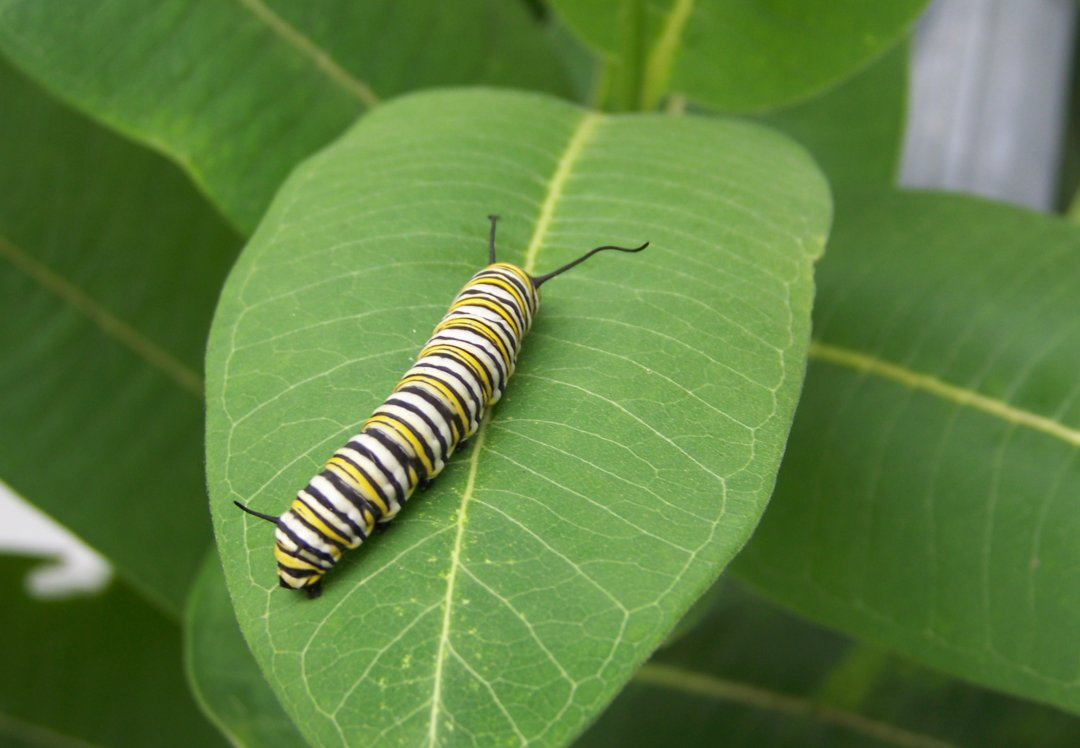
\includegraphics[width=\imsize]{./img/2746294525_52566921c8_o}
				\source{flic.kr/p/5bFtFB}{\ccbyncsa}
				}
			\only<2>{%
				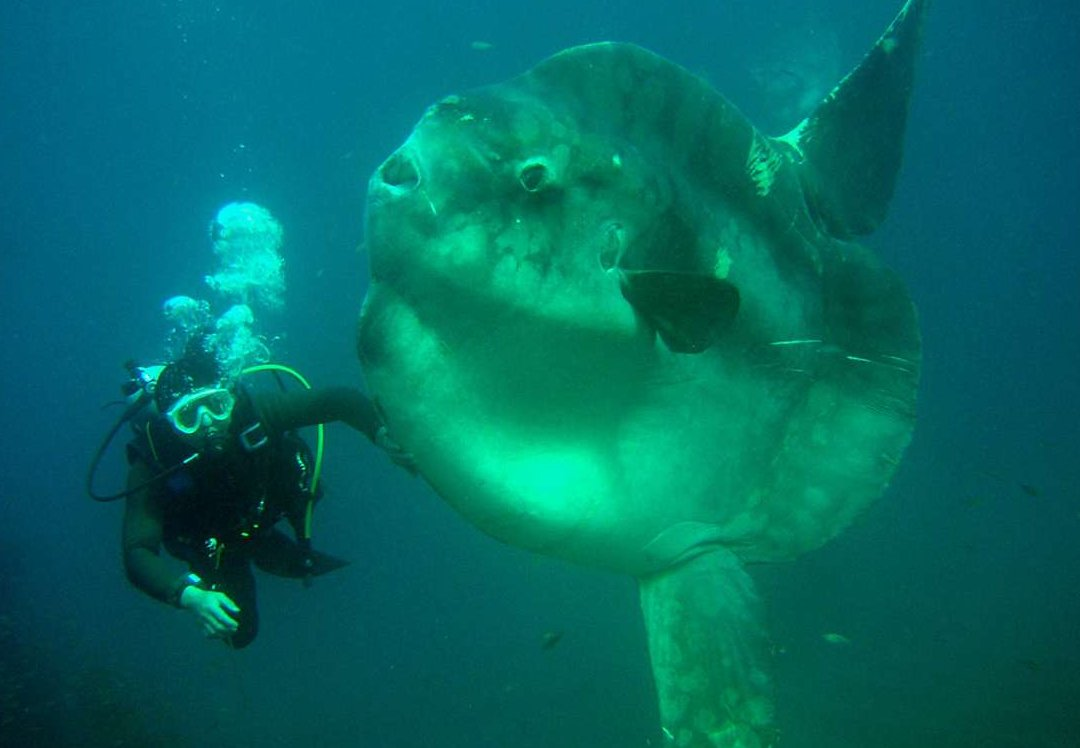
\includegraphics[width=\imsize]{./img/Bump_head_sunfish}%
				\source{enwp.org/molidae}{\ccbysa}
				}
			\only<3>{%
				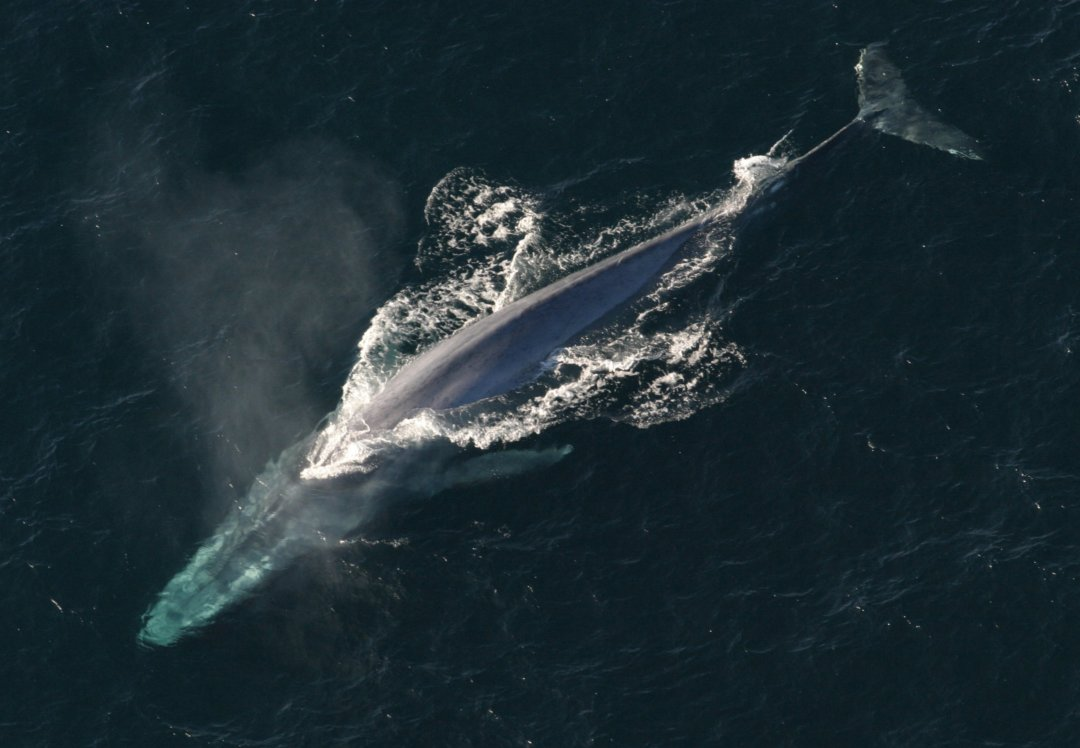
\includegraphics[width=\imsize]{./img/Anim1754_-_Flickr_-_NOAA_Photo_Library}%
				\source{enwp.org/bluewhale}{\ccPublicDomain}
				}
		\end{column}
	\end{columns}
\end{frame}

\begin{frame}
	\frametitle{Biology}
	% Image from https://teacheratsea.files.wordpress.com/2011/07/gills-an-o2.jpg
	\centering
	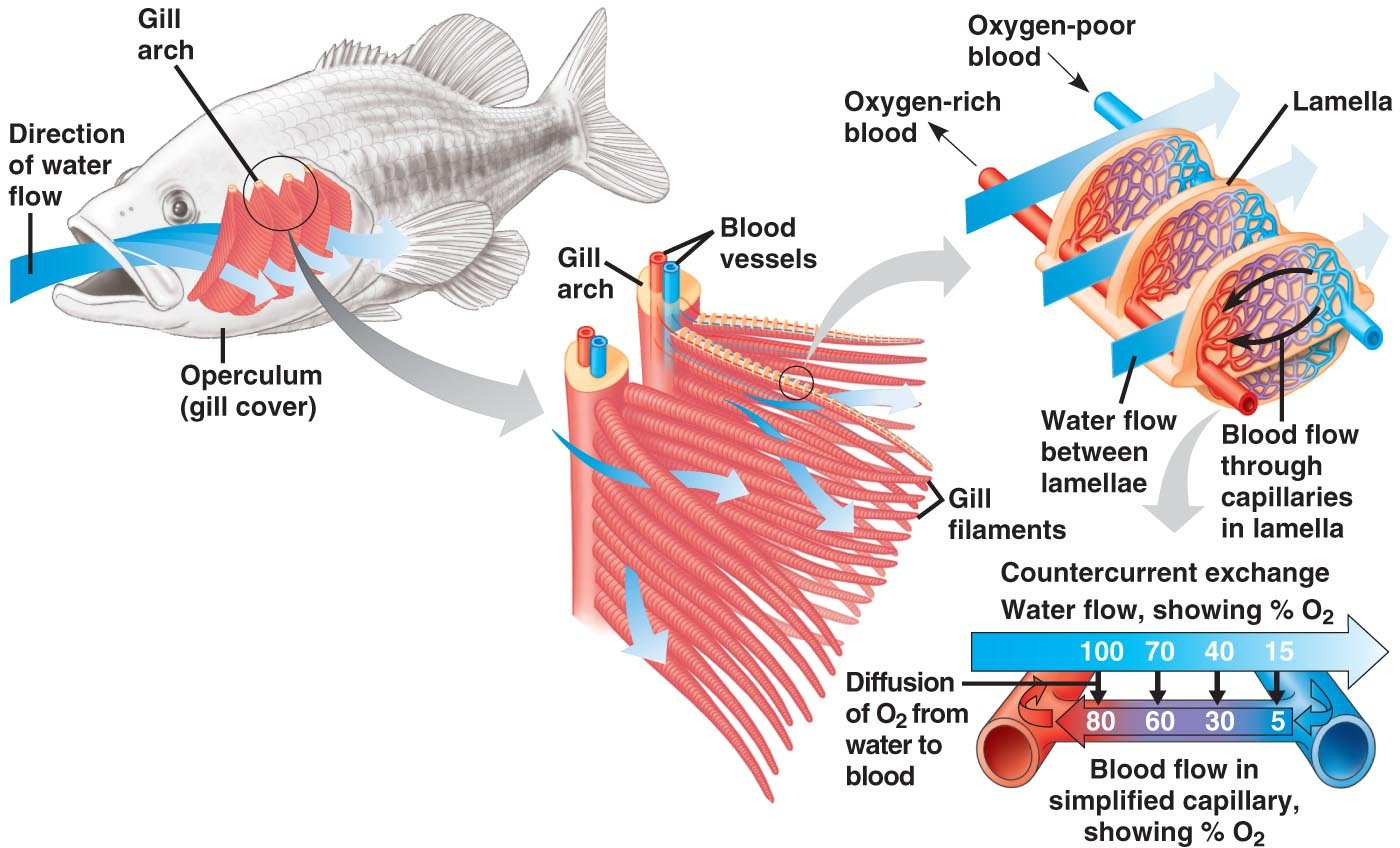
\includegraphics[width=0.618\linewidth]{./img/gills-an-o2}%
	\source{Campbell Biology: Concepts \& Connections}{\cite{Taylor2017}}
\end{frame}

\begin{frame}
	\frametitle{Adaptation}
	Adaptation to training exercise
	\begin{itemize}
		\item Increased body length and weight
		\item Skeletal and heart muscle hypertrophy
		\item Induction of angiogenesis in skeletal muscle
		\item Increase in haematocrit
	\end{itemize}
\end{frame}

\begin{frame}
	\frametitle{How?}
		\begin{columns}
	\begin{column}{0.618\linewidth}
		\begin{itemize}
			\item Fish training according to \textcite{Palstra2010}
			\item Scanning
			\item Delination
			\item Analysis
		\end{itemize}
	\end{column}
	\begin{column}{0.382\linewidth}
		\includegraphics<1>[width=\linewidth]{./img/0001713_swim-tunnel-5-l-230-v-50-hz}%
		\only<1>{\source{loligosystems.com/swim-tunnel-5-l-230-v-50-hz}{}}
		\includegraphics<2>[width=\linewidth]{./img/Anim1754_-_Flickr_-_NOAA_Photo_Library}%
		\only<2>{\source{This is just temporary!}{}}
		\end{column}	
	\end{columns}	
\end{frame}

\begin{frame}{movie}
	\centering    
	\movie[label=show3,
		width=\linewidth,
		poster,
		autostart,
		showcontrols,
		loop]{\includegraphics[width=1.0\textwidth]{./img/fishvideo.png}}{./img/fishvideo.mp4}
\end{frame}

\begin{frame}
	\frametitle{What?}
	\begin{itemize}
		\item Gill volume
		\item Gill complexity
	\end{itemize}
\end{frame}

\begin{frame}
	\frametitle{Wee!}
	\begin{itemize}
		\item We conclude that the zebrafish respiratory organ has a high plasticity, and after endurance training increases its volume and changes its structure in order to facilitate \ce{O2} uptake.
	\end{itemize}
\end{frame}

\begin{frame}
	\frametitle{Thanks!}
	\begin{columns}
		\begin{column}{0.618\linewidth}
		\begin{itemize}
			\item<1-> Team from the \emph{Topographic and clinical Anatomy} group
			\begin{itemize}
				\item<1-> Dea Aaldijk, Matthias Messerli
				\item<1-> Ruslan Hlushchuk, Valentin Djonov
				\item<1-> Fluri A.\ M.\ Wieland, Oleksiy Khoma
				\item<1-> Sarya Fark, Helena Röss
			\end{itemize}
			\item<1-> Other important people at the Institute of Anatomy
			\begin{itemize}
				\item<1-> Werner Graber, Jeannine Wagner-Zimmermann and Beat Haenni
				\item<1-> Regula Buergy, Eveline Yao and Sara Soltermann
				\item<1-> Marcos Sande, Carolina Garcia
				\item<1-> Ines Marquez, Xavier Langa and Alexander Uwe Ernst
			\end{itemize}
			\item<1-> SNF
			\item<2-> You, for listening
			\item<3-> Questions?
		\end{itemize}
		\end{column}
		\begin{column}{0.382\linewidth}
			\includegraphics<1->[width=\linewidth]{./img/team}
		\end{column}	
	\end{columns}	
\end{frame}

\begin{frame}
	\frametitle{References}
	%\renewcommand*{\bibfont}{\tiny}
	% No parentheses around the (empty) year: https://tex.stackexchange.com/a/147537
	%\renewcommand{\bibopenparen}{\addcomma\addspace}
	%\renewcommand{\bibcloseparen}{\addcomma\addspace}
	\setbeamertemplate{bibliography item}{\insertbiblabel}
	\printbibliography
\end{frame}

\begin{frame}
	\frametitle{Colophon}
	\begin{itemize}
		\item \href{http://intern.unibe.ch/dienstleistungen/corporate_design_und_vorlagen/praesentationen/index_ger.html}{Template from Corporate Design und Vorlagen, University of Bern}
		\item \href{https://github.com/habi/20190605_BrukerUserMeeting}{Full (\LaTeX) source code of this \textsc{beamer} presentation is available on GitHub}
	\end{itemize}
\end{frame}

\end{document}
